\chapter{Into The Matrix}

At its core, computational chemistry is basically matrix algebra applied to molecular systems. The performance of an algorithm, in other words its scaling, memory footprint and even accuracy, is intimately linked to how matrix operations and storage are handled internally. While the earliest implementations of molecular electronic structure methods often used hand-coded loops running over matrix indices, over the years, a whole ecosystem of matrix and tensor libraries has emerged in an attempt to lessen the burden of programmers, to various degrees of success, each with their strong and weak points. Choosing the best library for an algorithm is a non-trivial task, and depends on various factors: if memory is the bottle-neck, a sparse matrix library might be able to sufficiently compress data into a smaller space. If speed is the greatest concern, using targeting different archituectures like distributed memory systems, accelerators, or both, might be the solution. -.... The modern theoretical chemist needs to be aware of the possibilities ....

This chapter introduces basic concepts of matrix and tensor algebra, with a focus on storage orders. After introducing the core concepts, an (incomplete) list of matrix libraries is provided with small examples on how to use them. 

\section{Linear Algebra}

Linear algebra is a crucial tool in many areas of computational science, such as image processing, machine learning, computational physics, computational biology and of course computational chemistry. The most important concepts are discussed in this section, and generalized to tensors. Until mentioned otherwise, zero-based indexing is assumed. 

\subsection{Matrices}

A matrix is a rectangular, 2-dimensional array of dimension $M$ by $N$, containing a set of complex or real numbers $\{a_{ij}\}$ with ordered subscripts $i = 0,1,2,...M$ and $j = 0,1,2,...,N$, of the form
\begin{equation}
\mbf{A} = \begin{pmatrix}
a_{00} & a_{01} & \ldots & a_{0N} \\
a_{10} & a_{11} & \ldots & a_{1N} \\
\vdots & \vdots & \ddots & \vdots \\
a_{M0} & a_{M1} & \ldots & a_{MN}
\end{pmatrix}
\end{equation}
\noindent with $M$ \emph{rows} and $N$ \emph{columns}. \emph{Row vectors} and \emph{column vectors} are a type of matrix that contain only one row or one column, respectively. 

Matrix multiplication is only defined between matrices of dimension $M$ by $K$ and $K$ by $N$. The product yields an $M$ by $N$ matrix
\begin{align}
\mbf{C}_{M\times N} &= \mbf{A}_{M\times K} \mbf{B}_{K\times N} \\
c_{ij} = \sum_k a_{ik} b_{kj}
\end{align}

A matrix with an equal number of rows and columns is called a \emph{square matrix}. There a different types of square matrices:
\begin{enumerate}
\item \emph{Diagonal matrices} only have non-zero entries on the diagonal
\begin{equation}
a_{ij} = a_{ii} \delta_{ij}
\end{equation}

\item If all entries below the diagonal are zero, the matrix is \emph{lower triangular}. Similarly, if all elements above the diagonal are zero, the matrix is \emph{upper triangular}. Furthermore, if the diagional entries are all equal to 1, the matrix is \emph{unit triangular}.

\item The \emph{identity} or \emph{unit} matrix $\mbf{1}$ is defined as
\begin{align}
\mbf{A} \mbf{1} &= \mbf{1} \mbf{A} \\
\mbf{1}_{ij} = \delta_{ij}
\end{align} 

\item The \emph{inverse} of a matrix $\mbf{A}$ is defined as
\begin{equation}
\mbf{A}^{-1} \mbf{A} = \mbf{1}
\end{equation} 
\noindent It only exists for matrices with a non-zero determinant. If a matrix is non-invertible, it is also called \emph{singular}. 

\item A matrix is \emph{unitary}, if its inverse is equal to its conjugate transpose 
\begin{equation}
\mbf{A}^{-1} = \mbf{A}\pdg
\end{equation}
\noindent A real unitary matrix is called \emph{orthogonal}

\item A \emph{hermititan} matrix is its own conugate transpose
\begin{align}
\mbf{A} &= \mbf{A}\pdg \\
a_{ij} = (a_{ji})^*
\end{align}
\noindent A real hermitian matrix is called \emph{symmetric}

\item A hermitian matrix is said to be \emph{positive definite} if all of its eigenvalues are positive, and \emph{negative definite} if all eigenvalues are negative. \emph{Semi-definite} matrices additionally have some eigenvalues which are equal to zero.   
\end{enumerate}

Decompositions?

\section{Matrix Storage Formats}

The main memory in a computer, i.e. DRAM, is a linear address space and can be seen as a single, contiguous, one-dimensional array. Two-dimensional arrays like matrices need to be \emph{mapped} to this linear space by the compiler. This mapping depends on whether a dense or sparse view of the matrix is desired. 

\subsection{Dense Storage}

There are two ways to map a dense matrix to memory: row-major ordering and column-major ordering. The two storage orders differ by the order inwhich the individual elements are stored in memory (Figure ...). For an $M$ by $N$ matrix stored in a linear array $a$ in row-major format, the address offset of an element $a_{ij}$ compared to element $a_{00}$ is given by
\begin{equation}
A(i,j) \rightarrow \text{a[i * N + j]}
\end{equation}
\noindent and in column-major format by
\begin{equation}
A(i,j) \rightarrow \text{a[i + j * M]}
\end{equation}
Neither storage order has any advantages or disadvantes over the other one. It is only a matter of convention, and depend on the library and programming language. Fortran arrays are column-major, while C/C++ arrays are row-major. 

However, algorithms optimized for column-major access might not give the same performance for row-major formats and vice-versa. Consider a simple loop over matrix elements in the Fortran programming language
\begin{fortran}{Matrix Loop \label{FORTRAN1}}
DO i = 1, N
 DO j = 1, N
  A(i,j) = A(i,j) + 2
 ENDDO
ENDDO
\end{fortran}
\noindent By first looping over the rows, and then over the columns, the elements in the column-major matrix are accessed in a \emph{non-contiguous} manner. This prevents efficient optimizations like vectorization due to cache misses. By swapping the loops, the inner loop can be vectorized. Therefore, if algorithms assume a certain ordering, it is important to pass matrices of the same ordering.

Column-major ordering is by far the most common in scientifc computing. Matrix algebra routines like the QR, Eigenvalue or Cholesky decompositions are most intuitively written using column operations rather than row operations. Examples include the LAPACK and Eigen matrix libraries. 

\subsection{Sparse Storage}

A matrix is called \emph{sparse} if "most" of its elements are zero. The threshold between sparse and dense is ill-defined, and range anywhere between 1\% and 10\%. Sparse matrices are encountered in many fields of computational science in systems with few pair-wise interactions. By storing and looping over the siginifcant elements only, the memory footprint and the scaling of matrix multilications or decompositions can be significantly reduced. There are several different sparse matrix formats available. The following sections will demonstrate how the matrix
\begin{equation*}
\begin{pmatrix}
3 & 5 & 0 & 0 \\
0 & 4 & 0 & 0 \\
0 & 0 & 1 & 2 \\
0 & 0 & 6 & 7 
\end{pmatrix}
\end{equation*}
\noindent may be represented using some of these formats.

\subsubsection{Coordinate Format}

The coordinate format (COO) is one of the simplest storage schemes for sparse matrices. The matrix is stored using three arrays of lenghth $NNZ$ (number of non-zero elements) containing the row indices, column indices and matrix entries. The above matrix reduces to 
\begin{equation*}
COO: \left\lbrace
\begin{matrix}
\textrm{idx\_i} &= &\left[ 0, 0, 1, 2, 3, 2, 3 \right] \\
\textrm{idx\_j} &= &\left[ 0, 1, 1, 2, 2, 3, 3 \right] \\
\textrm{val}   &= &\left[ 3, 5, 4, 1, 6, 2, 7 \right] \\
\end{matrix}
\right.
\end{equation*}
\noindent The values do not need to be necessarily ordered. The COO format has the advantage that it is very easy to insert elements and change the sparsity pattern with low overhead. COO is generally not used for algebra due to slow random access of elements if elments are not in order. Rather, COO is an intermediate format for incremental construction of sparse matrices in the CSR or CSC format.

\subsubsection{Compressed Sparse Row}

The compressed sparse row format (CSR) is similar to COO, but compresses the rows. A CSR matrix is represented by three arrays: the extent of rows, the coulmn indices and non-zero matrix entries, with dimension $M$, $NNZ$ and $NNZ$ respectively. For the example matrix above, the CSR format gives
\begin{equation*}
CSR: \left\lbrace
\begin{array}{lll}
\textrm{row\_ext} &= &\left[ 0, 2, 3, 5 \right] \\
\textrm{col\_idx} &= &\left[ 0, 1, 1, 2, 2, 3, 3 \right] \\
\textrm{val}  &= &\left[ 3, 5, 4, 1, 2, 6, 7 \right] \\
\end{array}
\right.
\end{equation*}
\noindent The $i$th entry of the row extents contains the offset to the first non-zero element in the array \textrm{val} in the $i$th row. The entries in \textrm{col\_idx} are the associated column indices. Compared to COO, accessing elements is much faster, and the memory prefactor is reduced from $3NNZ$ to $2NNZE+M$. Matrix-vector products are very fast to compute, but CSR in not well suited for column slicing.

\subsubsection{Compressed Sparse Column}

The compressed sparse column format is the "column-major" analog to the CSR format. Instead of compressing the rows, it compresses the columns. The matrix in the CSC format is represented as

\begin{equation*}
CSC: \left\lbrace
\begin{array}{lll}
\textrm{col\_ext} &= &\left[ 0, 1, 3, 5 \right] \\
\textrm{row\_idx} &= &\left[ 0, 0, 1, 2, 2, 3, 3 \right] \\
\textrm{val}  &= &\left[ 3, 5, 4, 1, 6, 2, 7 \right] \\
\end{array}
\right.
\end{equation*}

CSC has similar performance to CSR, but is better suited for column slicing and therefore column-oriented matrix decomposition.

\subsection{Block Compressed Sparse Row}

The block-compressed sparse row (BCSR or BSR) format is a generalization of CSR. BCSR is ideal for matrices which are \emph{block-sparse}, i.e. matrices with few dense submatrices. For a constant block size $n$ by $m$, let the number of row and column blocks be $M_{blk}$ and $N_{blk}$, and $NNZ_{blk}$ the number of significant blocks. A matrix is then represented by three arrays containing the row block offsets, column block indices, and non-zero indices with size $M_{blk}$, $NNZ_{blk}$ and $NNZ_{blk}mn$. For blocks of size 2 by 2, the matrix above in the BCSR format yields

\begin{equation*}
BCSR: \left\lbrace
\begin{array}{lll}
\textrm{rowblk\_ext} &= &\left[ 0, 1 \right] \\
\textrm{colblk\_idx} &= &\left[ 0, 1 \right] \\
\textrm{val}  &= &\left[ 3, 0, 5, 4, 1, 6, 2, 7 \right] \\
\end{array}
\right.
\end{equation*}

\noindent The matrix is therefore split into two non-zero blocks of size 2-by-2 each, with elements $\{3,0,5,4\}$ and $\{1,6,2,7\}$ using column-major ordering. The BCSR format can further reduce the storage prefactor for block-sparse matrices. Smaller block-sizes can account for a higher degree of sparsity, but lead to a higher prefactor. Large block sizes have lower prefactor, but capture less of the sparsity. Figure \ref{fig:DISTSTOR2} shows the BCSR format for different split factors. The block sizes do not need to be the same, although a constant block size is best suited for load balancing. Whether a block is significant or not depends on the matrix norm that is chosen as a criterion for filtering. Popular choices include the Frobenius norm or the max norm. 

\subsection{Distributed Storage}

In distributed memory parallelism, processes do no longer have access to the whole matrix. The question then arises how to distribute data over multiple nodes or processes. Distribution can be \emph{blocked} or \emph{cyclic} (Figure \ref{fig:DISTSTOR1}). In the block representation, the matrix is distributed by dividing rows, columns (or both) by the number of processes, and distributing them sequentially over the processes. On the other hand, the cyclic representation distributes each individual row, column or matrix element over the set of processes and wrapping over them until all elements are assigned to a processor. The cyclic data layout achieves great load balancing by evenly distributing the matrix elements, but is not suitable for row or column manipulations due to a high communication overhead. A blocked representation can reduce this overhead, but load-balancing is more difficult to achieve if the number of elements is not evenly divisible by the number of processes. 

The most commonly used format for distributed matrix storage is the \emph{block-cyclic} representation (Figure \ref{fig:DISTSTOR2}). It combines the best of both worlds, with good load-balancing and low communication overhead for matrix algebra. Communication is most efficient by arranging processes into a 2-dimensional rectangular grid with $N_{proc} = N_{row} \times N_{col}$, such that each process is uniquely identifies by its coordinates $(i,j)$. A 4-by-2 grid therefore has 4 \emph{process rows} and 2 \emph{process columns}. With MPI, this is most easily achieved by using \emph{Cartesian grids}. In Cartesian grids, processes can only communicate with their nearest neighbor. 

Each process has a local array which can be packed in different ways. The ScaLAPACK library keeps the original ordering of the matrix elements, while other matrix libraries like DBCSR store the individual blocks sequentially in memory. Blocks do not necessarily need to be equal in size. Matrices like DBCSR also support heterogeneous block sizes.

All the sparse storage schemes discussed in the previous sections can also be applied to distributed matrices. DBCSR uses a block-sparse row format which distributes the significant blocks over the processors in a row-major format (Figure \ref{fig:DISTSTOR3}). 

\begin{figure}
\centering
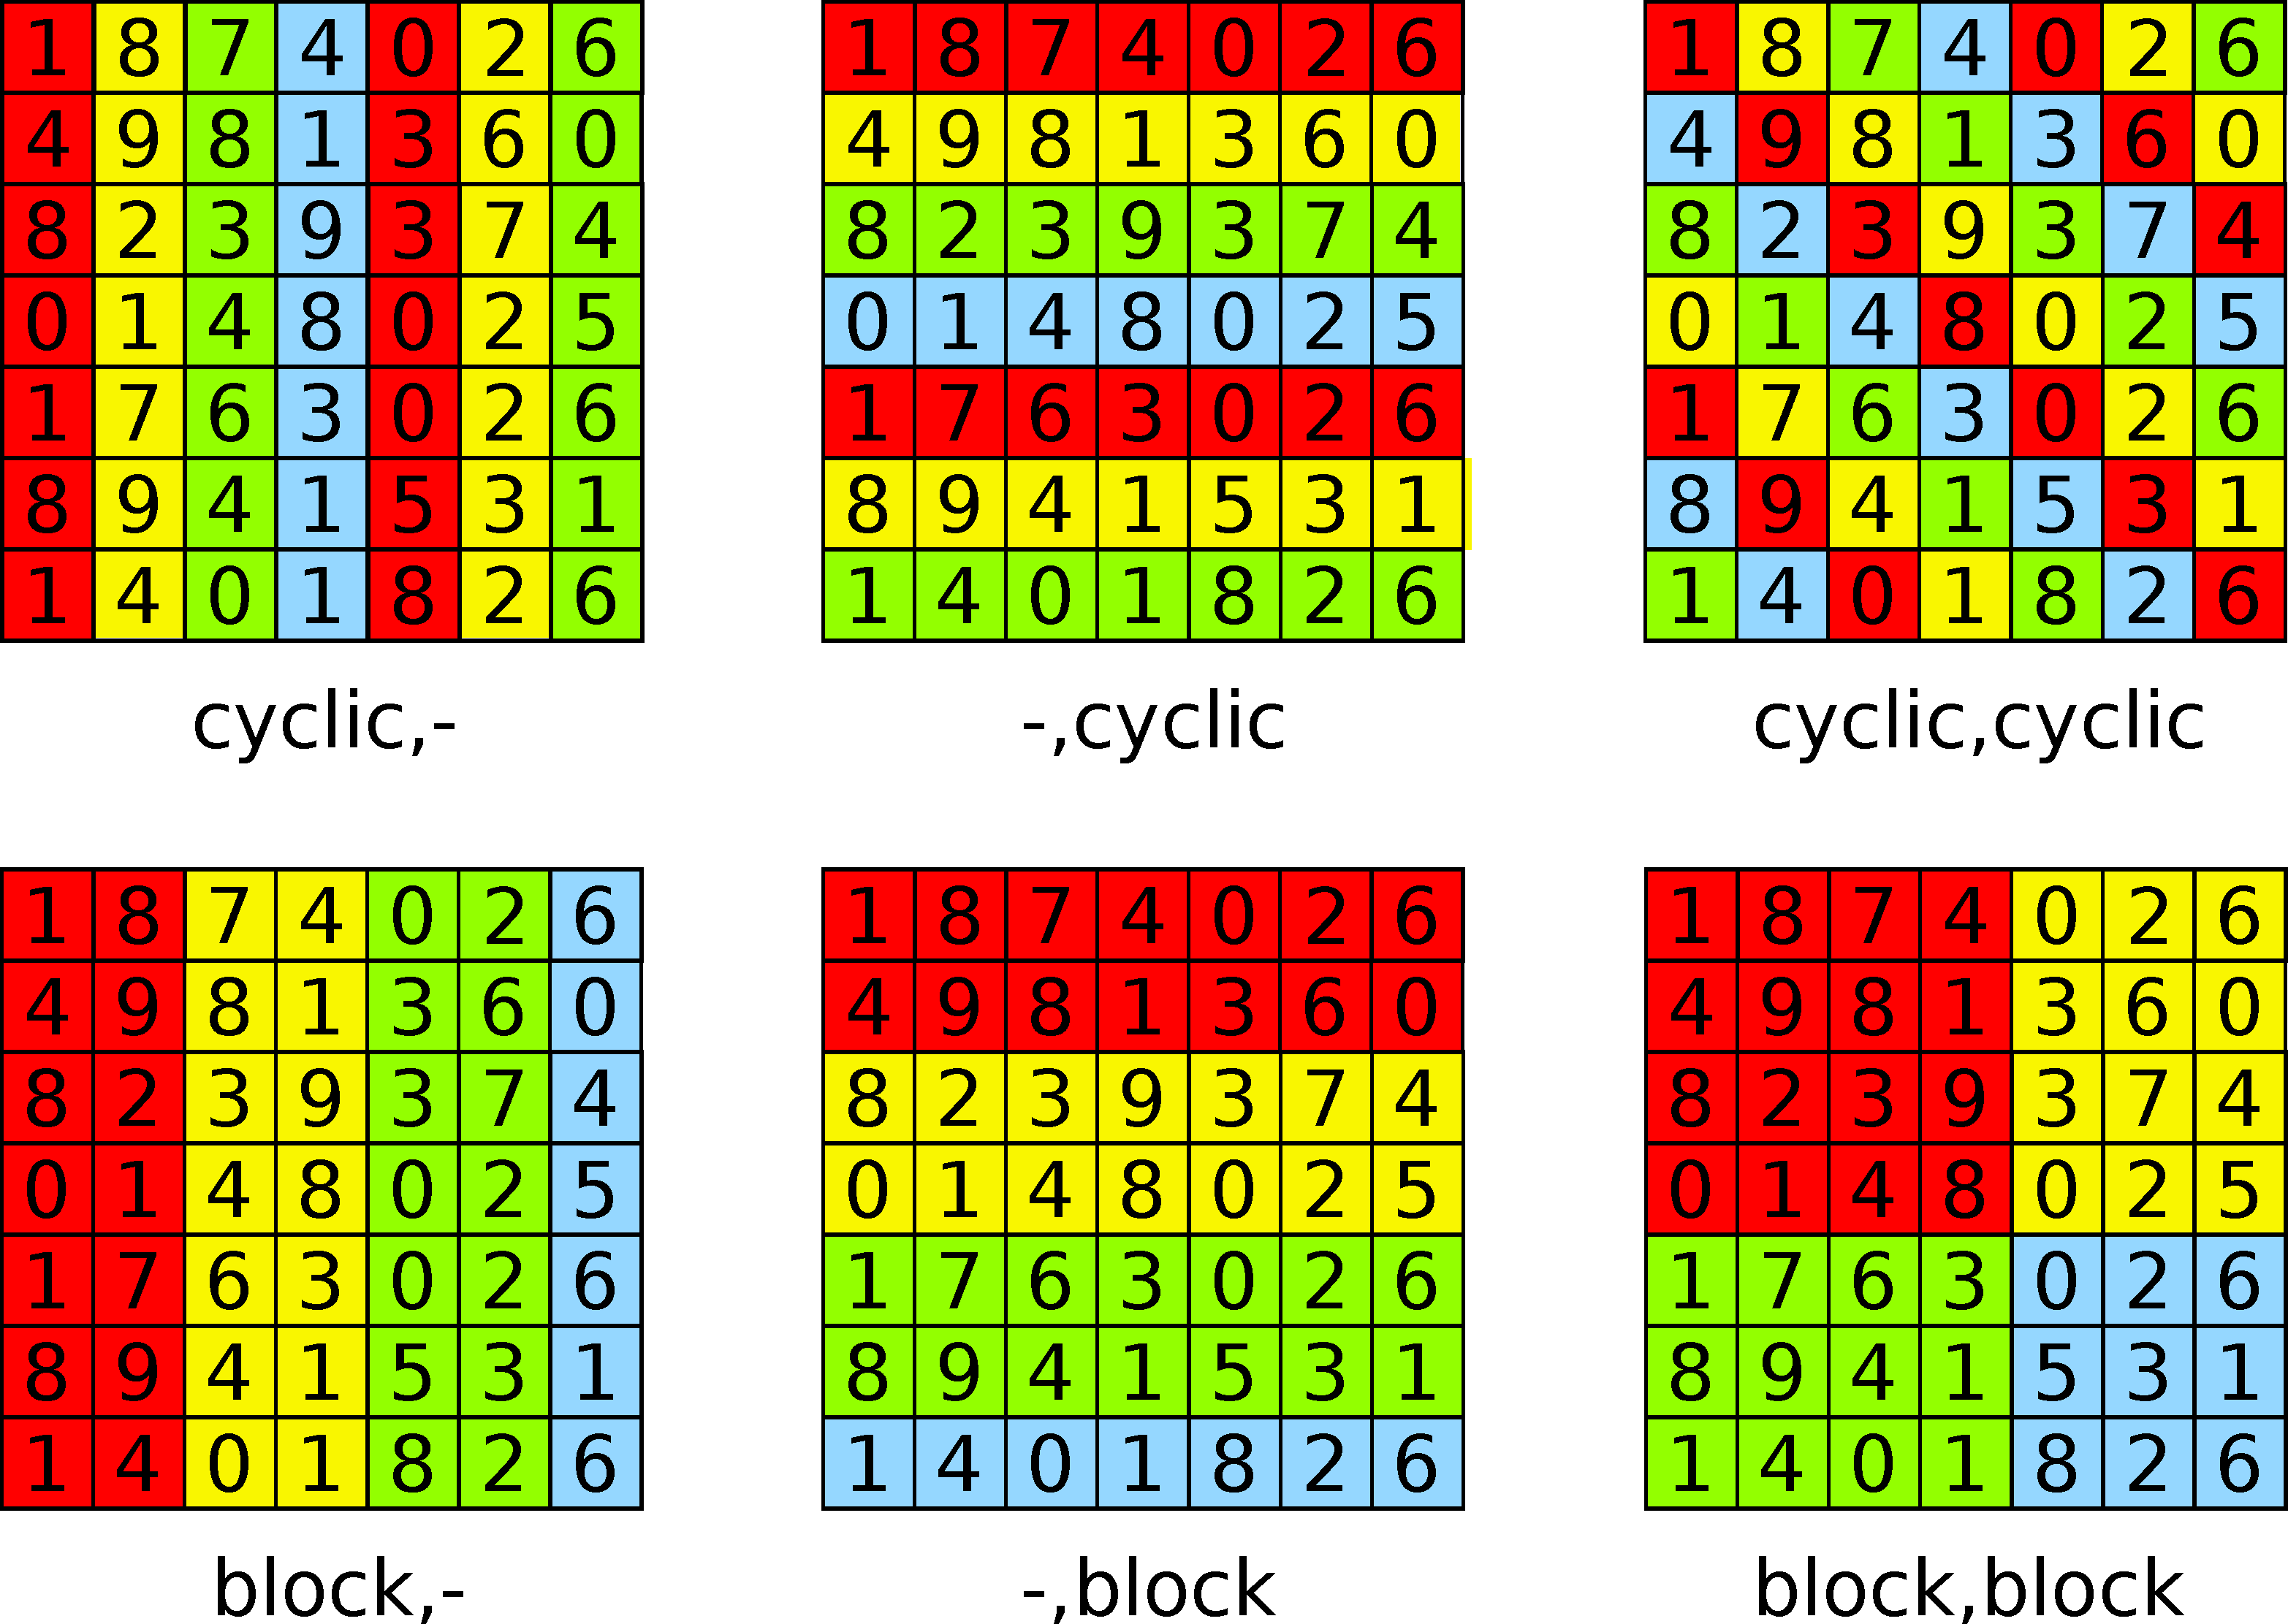
\includegraphics[scale=0.25]{Pics/DISTSTOR1.pdf}
\caption{There are two distinct ways to distribute rows, column or elements along processes, namely cyclic and block. Each color represents a processor (4 in total).}
\label{fig:DISTSTOR1}
\end{figure}

\begin{figure}
\centering
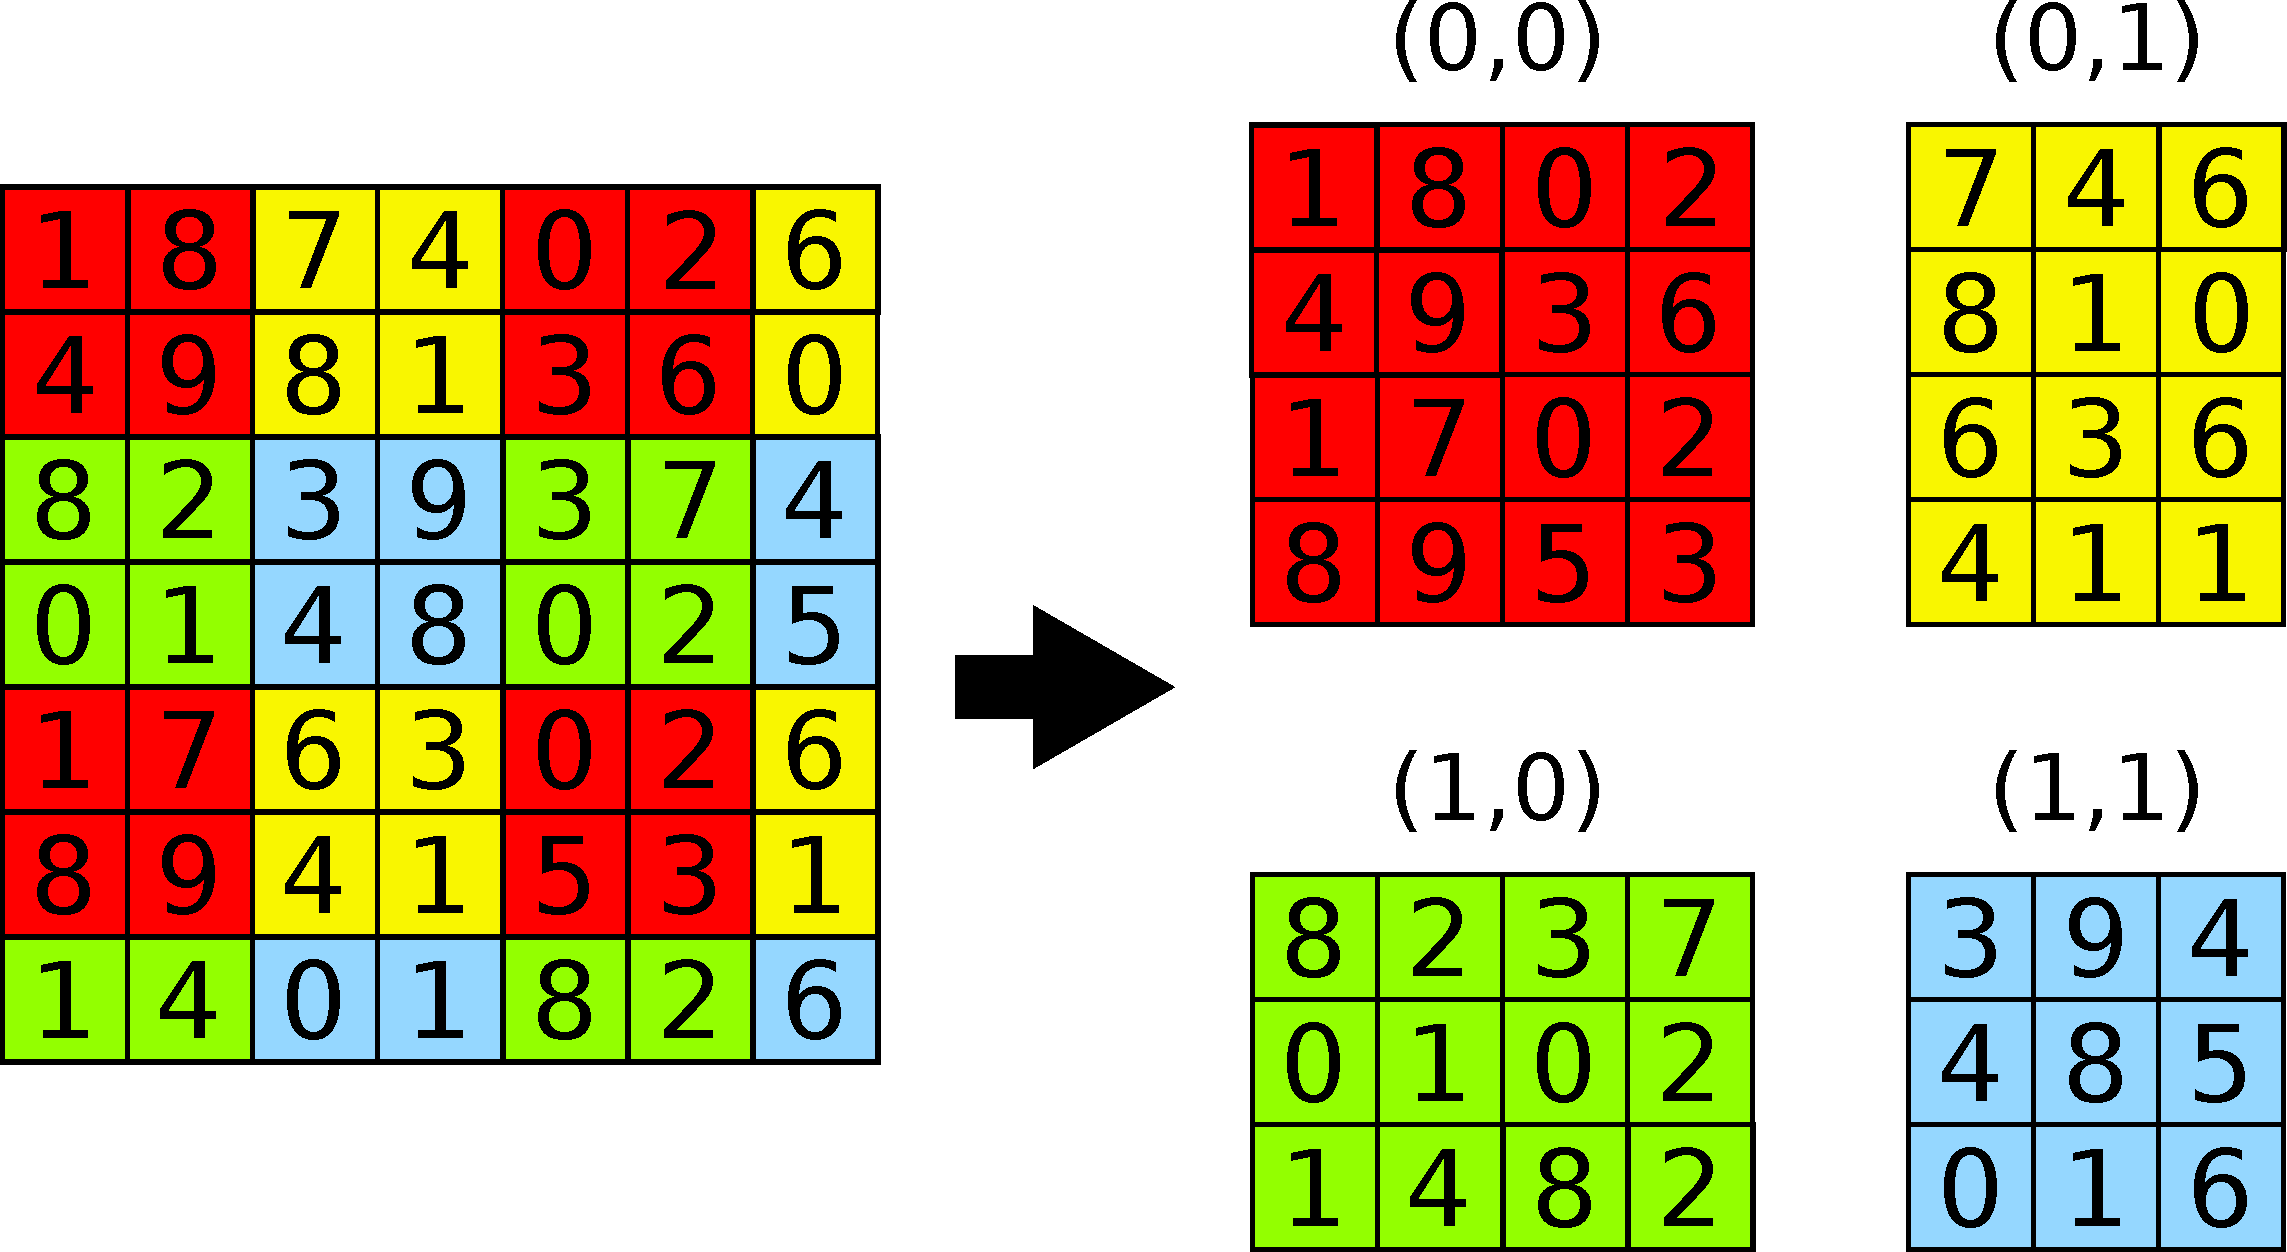
\includegraphics[scale=0.25]{Pics/DISTSTOR2.pdf}
\caption{In the block-cyclic distribution, the matrix is divided into blocks which are distributed over a processor grid, in this case 2 $\times$ 2.}
\label{fig:DISTSTOR2}
\end{figure}

\begin{figure}
\centering
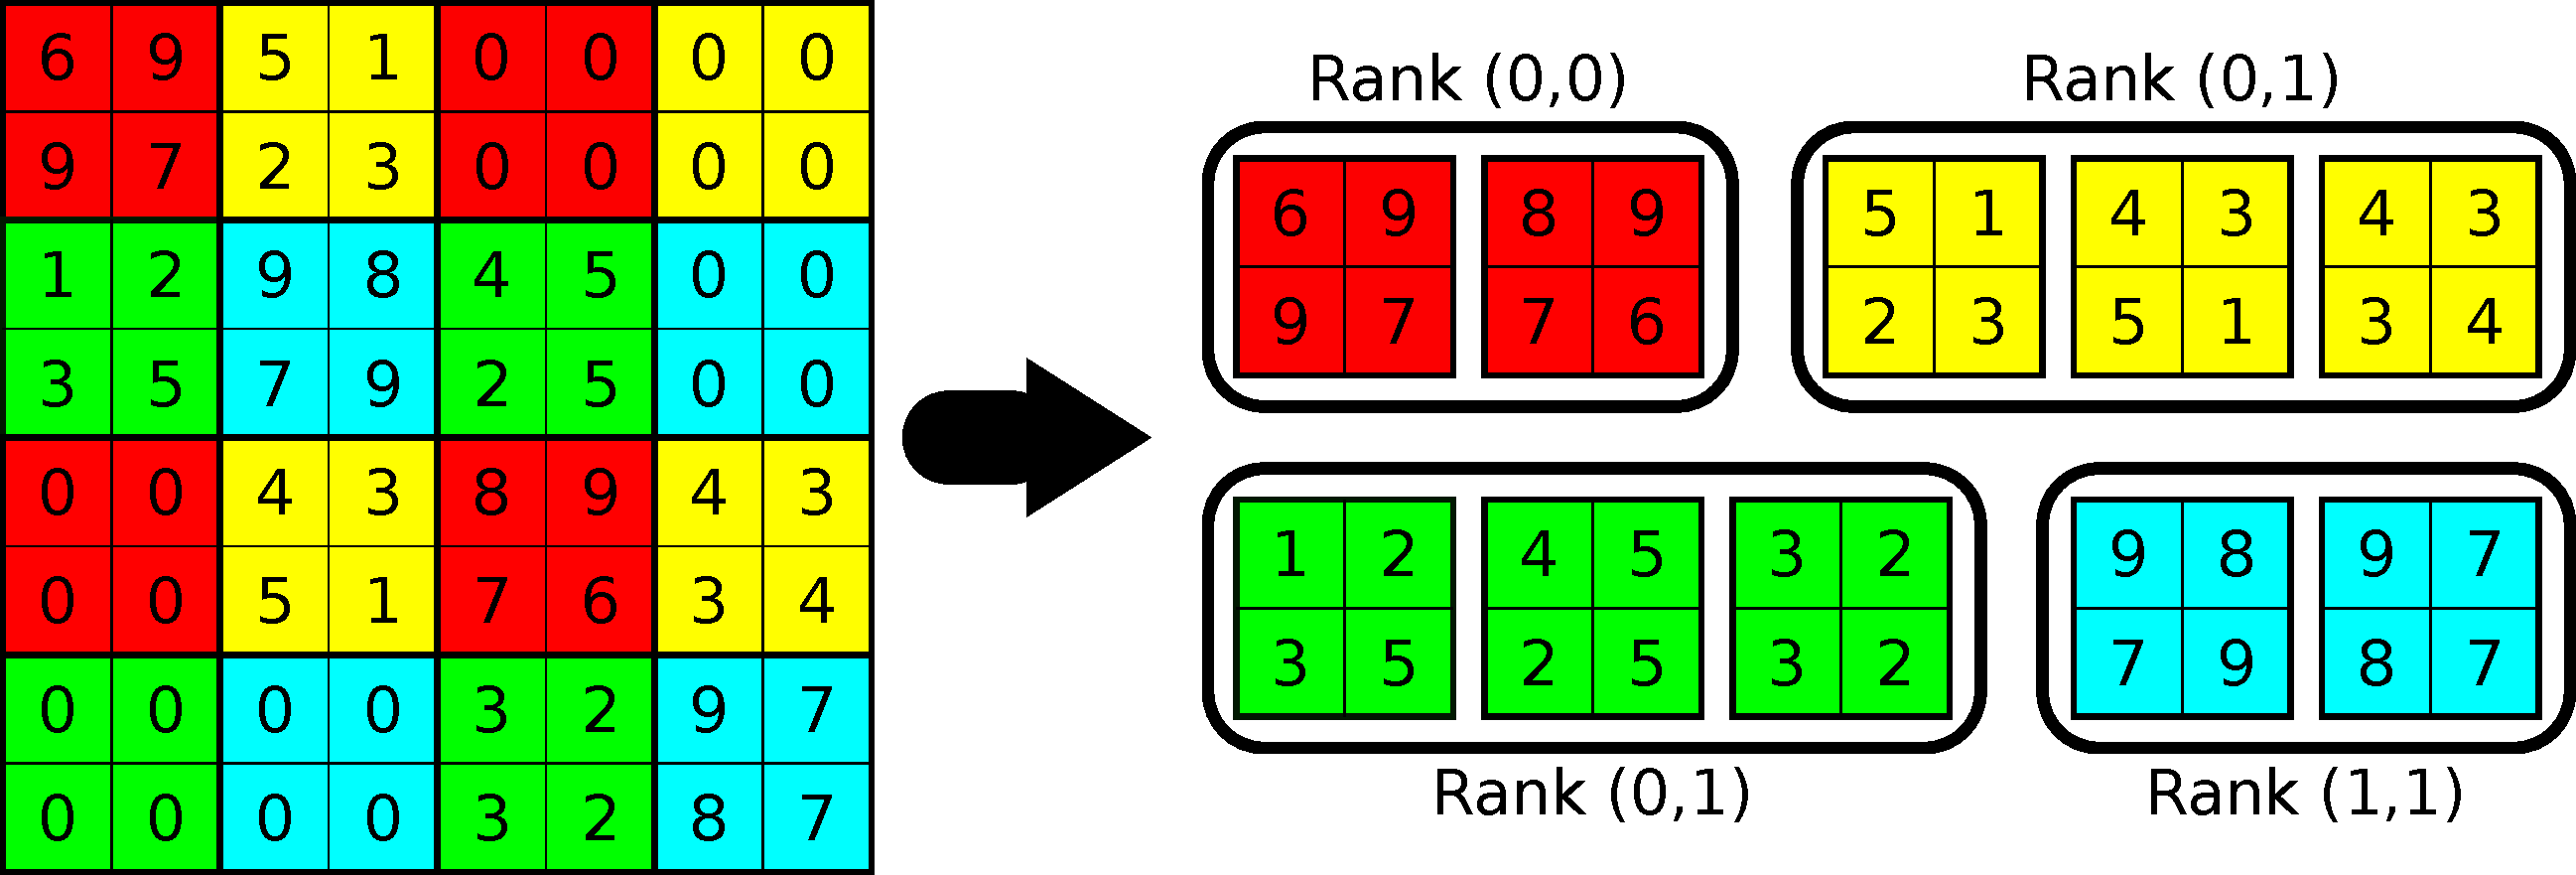
\includegraphics[scale=0.25]{Pics/DBCSR.pdf}
\caption{The DBCSR library distributes the significant blocks over the processor grid in row-major format.}
\label{fig:DISTSTOR2}
\end{figure}

%¨libxsmm?
%The block size has a major impact on the performance of distributed linear algebra algorithms. Consider the multiplication of two matrices. Multiplication can be reformulated in terms of individual multiplications of sub-blocks. 

\section{Tensors}

\subsection{Definitions}

Tensors are multi-dimensional arrays and can be seen as a generalization of matrix objects to higher dimensions, containing a set of complex or real values $\{a_{ijk...}\}$ with the ordered indices $i = 0,1,2,...N_0$, $j = 0,1,2,...N_1$, $k = 0,1,2,...N_2$ etc. The total number of indices required to identify an element in a tensor corresponds to its \emph{dimension}, also called \emph{rank}, \emph{order} or \emph{degree}. It should be stressed that tensor rank is different from the concept of a matrix rank. 

Tensors are important quantities in various scientific fields, especially in physics and quantum chemistry. Examples of tensor are the 4-dimensional MP2-amplitudes $t_{iajb}$ or the 3-dimensional 3c2e electron integrals. Matrices can be seen as 2-dimensional tensors. 

The analog of matrix multiplication is \emph{tensor contraction}, nd involves the summation over one or multiple indices. Consider for example the tensor contraction
\begin{equation}
C_{ijm} = \sum_{kl} A_{ikjl} B_{lkm}
\end{equation}
\noindent Here, the summation runs over the indices $kl$. Alternatively, the expression above can be abbreviated as
\begin{equation}
C_{ijm} = A_{ikjl} B_{lkm}
\label{eq:TENEX}
\end{equation}
\noindent which is known as  \emph{Einstein summation}, a notational convention used to simplify tensor expressions. Indices appearing on the right but not on the left are implicitly summed over. 

\subsection{Tensor Storage and Mapping}

Mapping multi-dimensional to the linear main memory is non-trivial. Tensors may follow a generalized column or row major storage such that
\begin{align}
A(i_0,i_1,...,i_n) &\rightarrow \sum_{k=0} \left( \prod_{l=k+1}^{N_{dim}} n_l \right) i_k \qquad \textrm{row-major} \\
A(i_0,i_1,...,i_n) &\rightarrow \sum_{k=0} \left( \prod_{l=0}^{k-1} n_l \right) i_k \qquad \textrm{column-major} 
\end{align} 
\noindent where $N_{dim}$ is the dimension of the tensor, and $n_k$ is the size of dimension $k$.

Consider again the tensor contraction \ref{eq:TENEX}.  loops running over the indices $kl$:
\begin{fortran}{Tensor Loop \label{lst:TLOOP}}
DO i = 1, ndim_i
  DO j = 1, ndim_j
    DO m = 1, ndim_m
      DO k = 1, ndim_k
        DO l = 1, ndim_l
          C(i,j,m) = A(i,k,j,l) * B(l,k,m)
        ENDDO
      ENDDO
    ENDDO
  ENDDO
ENDDO
\end{fortran}
\noindent Similarly to Example \ref{FORTRAN1} which loops over matrix elements, efficient parallelization by means of vectorization is a major concern when coding tensor contractions by hand. Ideally, tensor contractions should be offloaded to a specialized library. However, writing a general tensor library is a complex task, as the optimal kernel is dependent on the nature of the tensor contraction, i.e. number of indices involved, tensor dimensions and memory mapping. Whereas the \textrm{dgemm} BLAS routine only needs to know whether the matrices are transposed or not, the rapidly increasing number of parameters and loops makes it very difficult to write optimized code for arbitrary tensor contractions. For the example above, there are already $5!$ = $120$ different ways to arrange the loops.  

Many tensor libraries solve this problem by mapping tensors to matrices so that existing code for optimized matrix-matrix multiplication can be used instead. Consider the tensor $A_{ikjl}$. By introducing the \emph{super-indices} $P$ and $Q$, the tensor can be mapped to a matrix with $N_P$ = $n_i n_k$ rows and $N_Q$ = $n_j n_l$ columns with
\begin{align}
P(i,k) &= i + k*n_i \\
Q(j,l) &= j + l*n_j
\end{align}
\noindent The individual tensor elements are then accessed by
\begin{equation}
A(i,k,j,l) \rightarrow P(i,k) + Q(j,l) N_P
\end{equation}
\noindent using column-major storage for both the indices and super-indices. This corresponds to mapping $ik$ to the rows and $jl$ to the columns of a large matrix, which may also be written in a condensed notation as $\cn{01}{23}$, where $0,1,...$ indicate the mapping of the first, second, ... index of the tensor. As another example, consider the mapping $\cn{0}{213}$: this indicates that the index $i$ is mapped to rows, and $jkl$ are mapped to the columns. Alternatively, the mapping can be indicated by using upper or lower indices. $\cn{01}{23}$ corresponds to $A_{ik}^{jl}$ and $\cn{0}{213}$ to $A_{i}^{jkl}$. The lower indices are also known as \emph{covariant} indices, and the upper indices as \emph{contravariant} indices. From here on out, only the notation $\cn{\cdot}{\cdot}$ will be used.

Coming back to the tensor contraction in \ref{eq:TENEX}, mapping the tensors according to $A_{ikjl}^{\cn{02}{13}}$, $B_{lkm}^{\cn{10}{2}}$ and $C_{ijm}^{\cn{01}{2}}$, the contraction can be reformulated as a simple matrix multiplication
\begin{equation}
\mbf{C} = \mbf{A} \mbf{B}
\end{equation}
\noindent and optimized matrix libraries can be used to perform the tensor contraction. It is also possible to choose the mapping $B_{lkm}^{\cn{2}{10}}$, and the tensor contraction may be expressed as
\begin{equation}
\mbf{C} = \mbf{A} \mbf{B}^T
\end{equation}
\noindent by taking the transpose of $\mbf{B}$. In general, any tensor contraction can be reformulated as a matrix multiplication by mapping the indices which are summed over to either the row or column of a matrix, and the indices which are not involved to the remaining dimension. 

There are two drawbacks to this approach: first, tensors which are participating in different types of tensor contractions may need to be reordered. Reordering can take up a significant amount of time and add overhead to the tensor contraction, and it effectively doubles the amount of space needed by the tensor. Second, standard matrix libraries may not be optimized to handle tall-and-skinny (TAS) matrices. TAS matrices are matrices where one dimension is much larger then the other one, which is often the case for tensors with uneven mappings. Consider the tensor  $B_{lkm}^{\cn{10}{2}}$. It maps to a matrix with $n_kn_l$ rows and $n_m$ columns. If this matrix is distributed over an MPI grid, the process columns have much more work to perform than the process rows, which may lead to load imbalances. This problem can be addressed by dividing the TAS matrices up into multiple square chunks to improve load balancing, but adds further complexity during implementations.

\section{Matrix Libraries}

\subsection{BLAS}

\subsection{LAPACK}

\subsection{Eigen}

\subsection{ScaLAPACK}

canons algorithm

\subsection{DBCSR}

layers: cannon, rec, scheduler, small mm, gpus, etc.

rank, semi-definiteness etc ....

Storage: dense (shared), dense (dist), sparse (shared), sparse (dist)

Libraries: LAPACK, Eigen, ScaLAPACK